\documentclass[10pt]{article}
\usepackage[utf8]{inputenc}
\usepackage[T1]{fontenc}
\usepackage{amsmath}
\usepackage{amsfonts}
\usepackage{amssymb}
\usepackage[version=4]{mhchem}
\usepackage{stmaryrd}
\usepackage{graphicx}
\usepackage[export]{adjustbox}
\graphicspath{ {./images/} }

\begin{document}
\section*{Flight Mechanics Review}
\section*{a) General Rigid Body Dynamics Equations in 3D (12 Equations)}
A rigid body in 3D is fully described by 12 equations, split equally into 6 kinetic (dynamics) and 6 kinematic (geometric) equations.

\section*{Kinetic Equations (Dynamics)}
These equations govern the forces and moments acting on the body.

\section*{Translational Dynamics (Newton's Second Law)}
(1)

$$
\dot{u}=\left(F_{\mathrm{x}} / m\right)+r \cdot v-q \cdot w
$$

(2)

$$
\dot{v}=\left(F_{\gamma} / m\right)+p \cdot w-r \cdot u
$$


\begin{equation*}
\dot{w}=(F z / m)+q \cdot u-p \cdot v \tag{3}
\end{equation*}


\section*{Where:}
\begin{itemize}
  \item $u, v, w=$ Velocity components along the body $x-, y-$, and $z$-axes
  \item $F_{\mathrm{x}}, F_{\gamma}, F z=$ External force components along the body axes
  \item $m=$ Mass of the body
  \item $p, q, r=$ Angular velocity components about the body x -, y -, and z -axes
\end{itemize}

\section*{Rotational Dynamics (Euler's Equations)}
(4):

$$
\dot{p}=\left(1 / I_{\mathrm{x}}\right) \cdot\left[M_{\mathrm{x}}+\left(I_{\gamma}-I z\right) \cdot q \cdot r\right]
$$

(5):

$$
\dot{q}=\left(1 / I_{\gamma}\right) \cdot\left[M_{\gamma}+\left(I z-I_{\mathrm{x}}\right) \cdot r \cdot p\right]
$$

(6):

$$
\dot{r}=(1 / I z) \cdot\left[M z+\left(I_{\mathrm{x}}-I_{\gamma}\right) \cdot p \cdot q\right]
$$

Where:

\begin{itemize}
  \item $I_{\mathrm{x}}, I_{\gamma}, I z=$ Moments of inertia about the body axes
  \item $M_{\mathrm{x}}, M_{\gamma}, M z=$ External moment components about the body axes
\end{itemize}

\section*{Kinematic Equations (Geometry)}
These equations relate the velocities and angular rates to the changes in position and orientation.

\section*{Translational Kinematics (Position Updates)}
(7):

$$
\begin{aligned}
\dot{\mathrm{x}}=u \cdot \cos \theta \cdot & \cos \psi+v \cdot(\sin \varphi \cdot \sin \theta \cdot \cos \psi-\cos \varphi \cdot \sin \psi) \\
& +w \cdot(\cos \varphi \cdot \sin \theta \cdot \cos \psi+\sin \varphi \cdot \sin \psi)
\end{aligned}
$$

(8):\\
$\dot{\mathrm{y}}=u \cdot \cos \theta \cdot \sin \psi+v \cdot(\sin \varphi \cdot \sin \theta \cdot \sin \psi+\cos \varphi \cdot \cos \psi)$

$$
+w \cdot(\cos \varphi \cdot \sin \theta \cdot \sin \psi-\sin \varphi \cdot \cos \psi)
$$

(9):

$$
\dot{\mathrm{z}}=-u \cdot \sin \theta+v \cdot \sin \varphi \cdot \cos \theta+w \cdot \cos \varphi \cdot \cos \theta
$$

\section*{Where:}
\begin{itemize}
  \item $x, y, z=$ Inertial (earth-fixed) coordinates
  \item $\varphi, \theta, \psi=$ Euler angles (roll, pitch, yaw)\\
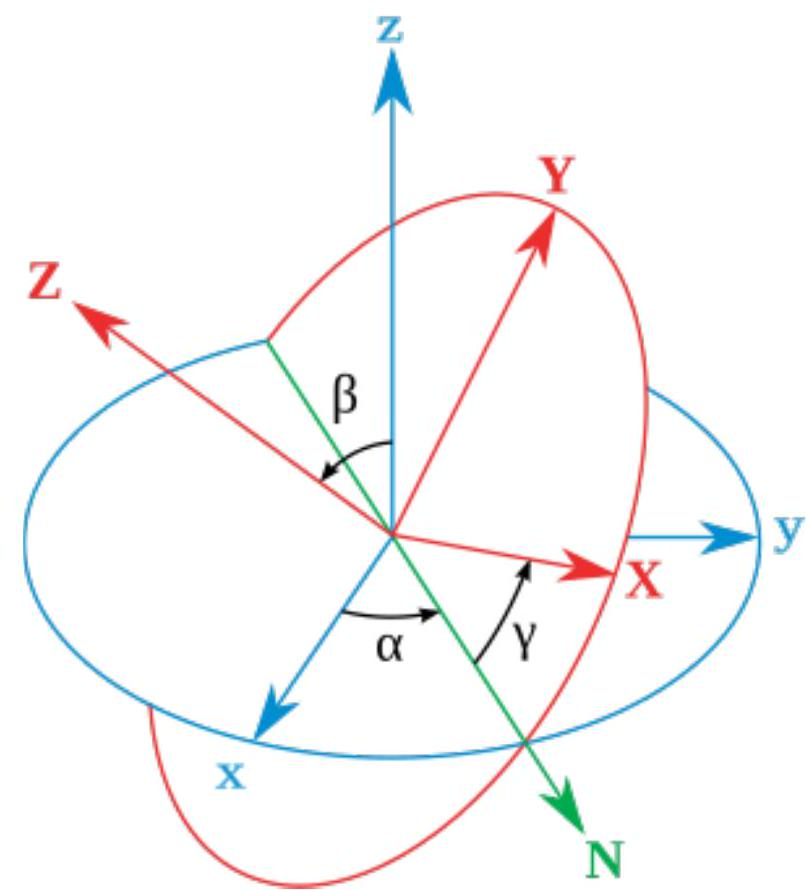
\includegraphics[max width=\textwidth, center]{2025_02_14_6d0761894995bbdc62abg-2}
\end{itemize}

Euler angles

\section*{Rotational Kinematics (Euler Angle Rates)}
(10):

$$
\dot{\varphi}=p+q \cdot \sin \varphi \cdot \tan \theta+r \cdot \cos \varphi \cdot \tan \theta
$$

(11):

$$
\theta=q \cdot \cos \varphi-r \cdot \sin \varphi
$$

(12):

$$
\psi=(q \cdot \sin \varphi+r \cdot \cos \varphi) / \cos \theta
$$

These 12 equations together comprehensively describe the motion of a rigid body in 3D space.

\section*{b) Classification into Kinetics and Kinematics \\
 Kinetic Equations (6 in total):}
\begin{itemize}
  \item Equations (1) - (3): Translational dynamics
  \item Equations (4) - (6): Rotational dynamics
\end{itemize}

Kinematic Equations (6 in total):

\begin{itemize}
  \item Equations (7) - (9): Relate body velocities (expressed in body frame) to inertial position changes
  \item Equations (10) - (12): Relate body angular rates to Euler angle rates
\end{itemize}

\section*{c) Additional Equations for Fixed-Wing Airplane Equations of Motion (EOM)}
To specialize the general RBD equations for a fixed-wing airplane, the following are added: •

\section*{Aerodynamic Force and Moment Models:}
Aerodynamic forces are expressed as functions of dynamic pressure, wing area, and non-dimensional coefficients (e.g., $C x, C y, C z$ ). Similarly, aerodynamic moments (roll $L$, pitch $M$, yaw $N$ ) are modeled using coefficients that depend on angle of attack, sideslip, and control surface deflections.

\section*{- Gravitational Force Projection:}
The weight of the airplane is resolved along the body axes via the transformation from the inertial (or earthfixed) frame.

\section*{- Velocity-to-Angle Relationships:}
Equations that relate the components of velocity in the body frame to the airspeed, angle of attack ( $\alpha$ ), and sideslip angle ( $\beta$ ).

\begin{itemize}
  \item Control Input Effects:
\end{itemize}

Additional relations that quantify how control surface deflections affect the aerodynamic forces and moments.

\section*{d) Assumptions in Deriving Airplane Equations of Motion.}
Common assumptions include:

\begin{itemize}
  \item Rigid Body Approximation: The aircraft is assumed not to deform.
  \item Constant Mass and Inertia: Effects of fuel burn or payload shifts are neglected.
  \item Quasi-Steady Aerodynamics: Aerodynamic forces and moments are assumed to respond instantaneously to changes in flight conditions.
  \item Small Perturbations: Linearization is often performed around a trim condition.
  \item Neglection of High-Order Effects: Compressibility, viscous effects, and higher-order nonlinearities are typically ignored in preliminary analyses.
  \item Uniform Atmospheric Conditions: The air is assumed to have steady and uniform properties.
\end{itemize}

\section*{e) Mathematical Classification of the Airplane EOM.}
\begin{center}
\begin{tabular}{|l|l|}
\hline
Order & The equations are represented as first-order differential equations in state-space form. \\
\hline
Type & \begin{tabular}{l}
They are Ordinary Differential Equations (ODEs), with time being the independent \\
variable. \\
\end{tabular} \\
\hline
Linearity & \begin{tabular}{l}
The full equations are nonlinear, although linearization is common near steady flight \\
conditions. \\
\end{tabular} \\
\hline
\end{tabular}
\end{center}

Coupling $\quad$ The equations are generally coupled, as translational and rotational dynamics interact. Under certain assumptions (such as decoupling of longitudinal and lateral-directional dynamics), the equations can be simplified to an uncoupled form.

\section*{f) Difference Between Body Axes and Earth (Inertial) Axes.}
\section*{- Body Axes:}
A coordinate system fixed to the airplane, typically defined as:

\begin{itemize}
  \item $\quad x$ - axis: along the fuselage (forward),
  \item $y$ - axis: towards the right wing,
  \item $z$-axis: downward.
\end{itemize}

The body axes rotate with the aircraft.

\begin{itemize}
  \item Earth (Inertial) Axes:
\end{itemize}

A fixed or quasi-fixed coordinate system relative to the Earth, often defined as North-East-Down (NED) or a similar scheme, serving as an absolute reference frame.

\section*{g) Difference Between Pitch Angle ( $\theta$ ) vs. Angle of Attack $(\alpha)$ and Sideslip Angle ( $\beta$ ) vs. Heading Angle ( $\psi$ ).}
\section*{- Pitch Angle ( $\theta$ ) vs. Angle of Attack ( $\alpha$ ):}
The pitch angle $\theta$ is the orientation of the aircraft's longitudinal axis relative to the horizon, while the angle of attack $\alpha$ is the angle between the chord line (or x-axis) and the oncoming airflow. In steady, coordinated flight these angles are related, but during maneuvers or in the presence of wind, they can differ significantly.

\section*{- Sideslip Angle ( $\beta$ ) vs. Heading Angle ( $\psi$ ):}
The sideslip angle $\beta$ is the angle between the aircraft's longitudinal axis and the relative wind, whereas the heading angle $\psi$ is the navigational direction of the aircraft relative to a fixed reference (such as geographic North).

\section*{h) Attitude Representations: Advantages and Disadvantages}
\section*{- Euler Angles:}
\begin{itemize}
  \item Advantages: Intuitive (roll, pitch, yaw) and straightforward.
  \item Disadvantages: Suffer from singularities (gimbal lock) when, for example, the pitch angle approaches $\pm 90$.
\end{itemize}

\section*{- Direction Cosine Matrix (DCM):}
\begin{itemize}
  \item Advantages: No singularity issues and provides a full transformation matrix.
  \item Disadvantages: Requires 9 elements along with orthogonality constraints, which can complicate numerical implementation.
\end{itemize}

\section*{- Quaternions:}
\begin{itemize}
  \item Advantages: Compact (4 parameters), computationally efficient, and free from singularities.
  \item Disadvantages: Less intuitive and involve a double-cover issue (i.e., $q$ and -q represent the same orientation).
  \item Axis-Angle Representation:
  \item Advantages: Provides a clear geometric interpretation (rotation by a specific angle about a fixed axis).
  \item Disadvantages: Less practical for sequential rotations or for numerical integration when rotations are small.
\end{itemize}

\end{document}